\documentclass{article}

\usepackage{fancyhdr} % Required for custom headers
\usepackage{lastpage} % Required to determine the last page for the footer
\usepackage{extramarks} % Required for headers and footers
\usepackage[usenames,dvipsnames]{color} % Required for custom colors
\usepackage{graphicx} % Required to insert images
\usepackage{listings} % Required for insertion of code
\usepackage{courier} % Required for the courier font
\usepackage{lipsum} % Used for inserting dummy 'Lorem ipsum' text into the template
\usepackage{amsmath}
\usepackage{titlesec}
\usepackage{pgfgantt}

\setcounter{secnumdepth}{4}

\titleformat{\paragraph}
{\normalfont\normalsize\bfseries}{\theparagraph}{1em}{}
\titlespacing*{\paragraph}
{0pt}{3.25ex plus 1ex minus .2ex}{1.5ex plus .2ex}

% Margins
\topmargin=-0.45in
\evensidemargin=0in
\oddsidemargin=0in
\textwidth=6.5in
\textheight=9.0in
\headsep=0.25in

\linespread{1.01} % Line spacing

% Set up the header and footer
\pagestyle{fancy}
\lhead{\hmwkAuthorName} % Top left header
\chead{Progress Report 1} % Top center head
\rhead{February 5th 2016}
\lfoot{\lastxmark} % Bottom left footer
\cfoot{\ \thepage\ of\ \protect\pageref{LastPage}} % Bottom right footer
\renewcommand\headrulewidth{0.2pt} % Size of the header rule
\renewcommand\footrulewidth{0.4pt} % Size of the footer rule


%----------------------------------------------------------------------------------------
%	DOCUMENT STRUCTURE COMMANDS
%	Skip this unless you know what you're doing
%----------------------------------------------------------------------------------------

% Header and footer for when a page split occurs within a problem environment
\newcommand{\enterProblemHeader}[1]{
\nobreak\extramarks{#1}{#1 continued on next page\ldots}\nobreak
\nobreak\extramarks{#1 (continued)}{#1 continued on next page\ldots}\nobreak
}

% Header and footer for when a page split occurs between problem environments
\newcommand{\exitProblemHeader}[1]{
\nobreak\extramarks{#1 (continued)}{#1 continued on next page\ldots}\nobreak
\nobreak\extramarks{#1}{}\nobreak
}

\setcounter{secnumdepth}{0} % Removes default section numbers
\newcounter{homeworkProblemCounter} % Creates a counter to keep track of the number of problems

\newcommand{\homeworkProblemName}{}
\newenvironment{homeworkProblem}[1][Problem \arabic{homeworkProblemCounter}]{ % Makes a new environment called homeworkProblem which takes 1 argument (custom name) but the default is "Problem #"
\stepcounter{homeworkProblemCounter} % Increase counter for number of problems
\renewcommand{\homeworkProblemName}{#1} % Assign \homeworkProblemName the name of the problem
\section{\homeworkProblemName} % Make a section in the document with the custom problem count
\enterProblemHeader{\homeworkProblemName} % Header and footer within the environment
}{
\exitProblemHeader{\homeworkProblemName} % Header and footer after the environment
}

\newcommand{\problemAnswer}[1]{ % Defines the problem answer command with the content as the only argument
\noindent\framebox[\columnwidth][c]{\begin{minipage}{0.98\columnwidth}#1\end{minipage}} % Makes the box around the problem answer and puts the content inside
}

\newcommand{\homeworkSectionName}{}
\newenvironment{homeworkSection}[1]{ % New environment for sections within homework problems, takes 1 argument - the name of the section
\renewcommand{\homeworkSectionName}{#1} % Assign \homeworkSectionName to the name of the section from the environment argument
\subsection{\homeworkSectionName} % Make a subsection with the custom name of the subsection
\enterProblemHeader{\homeworkProblemName\ [\homeworkSectionName]} % Header and footer within the environment
}{
\enterProblemHeader{\homeworkProblemName} % Header and footer after the environment
}

%----------------------------------------------------------------------------------------
%	NAME AND CLASS SECTION
%----------------------------------------------------------------------------------------

\newcommand{\hmwkTitle}{Progress Report 1} % Assignment title
\newcommand{\hmwkDueDate}{Friday, 5th of February} % Due date
\newcommand{\hmwkClass}{Progress Report 1} % Course/class
\newcommand{\hmwkClassTime}{} % Class/lecture time
\newcommand{\hmwkClassInstructor}{} % Teacher/lecturer
\newcommand{\hmwkAuthorName}{Paul McGurk} % Your name

%----------------------------------------------------------------------------------------
%	TITLE PAGE
%----------------------------------------------------------------------------------------

\title{
\textmd{\textbf{Progress Report 1}}\\
}

\author{\textbf{\hmwkAuthorName}}

%----------------------------------------------------------------------------------------
\begin{document}
%\tableofcontents
\newpage

\section{Progress}
\subsection{Application Development}
\subsubsection{General}
The login page directs the user to the student/lecturer application depending on their account type. The application then uses the PHP session cookie to populate the application with the user's details and enrolled classes.

\subsubsection{Student Side}
In the student application, a list of enrolled classes appears on the welcome page, populated from the database. Clicking on one of these classes opens a list of lectures, also populated from the database, and clicking on one of these lectures will open a list of questions available for this class and lecture. Again, clicking on one of these questions will show a populated questions page including the button layout.

\begin{center}
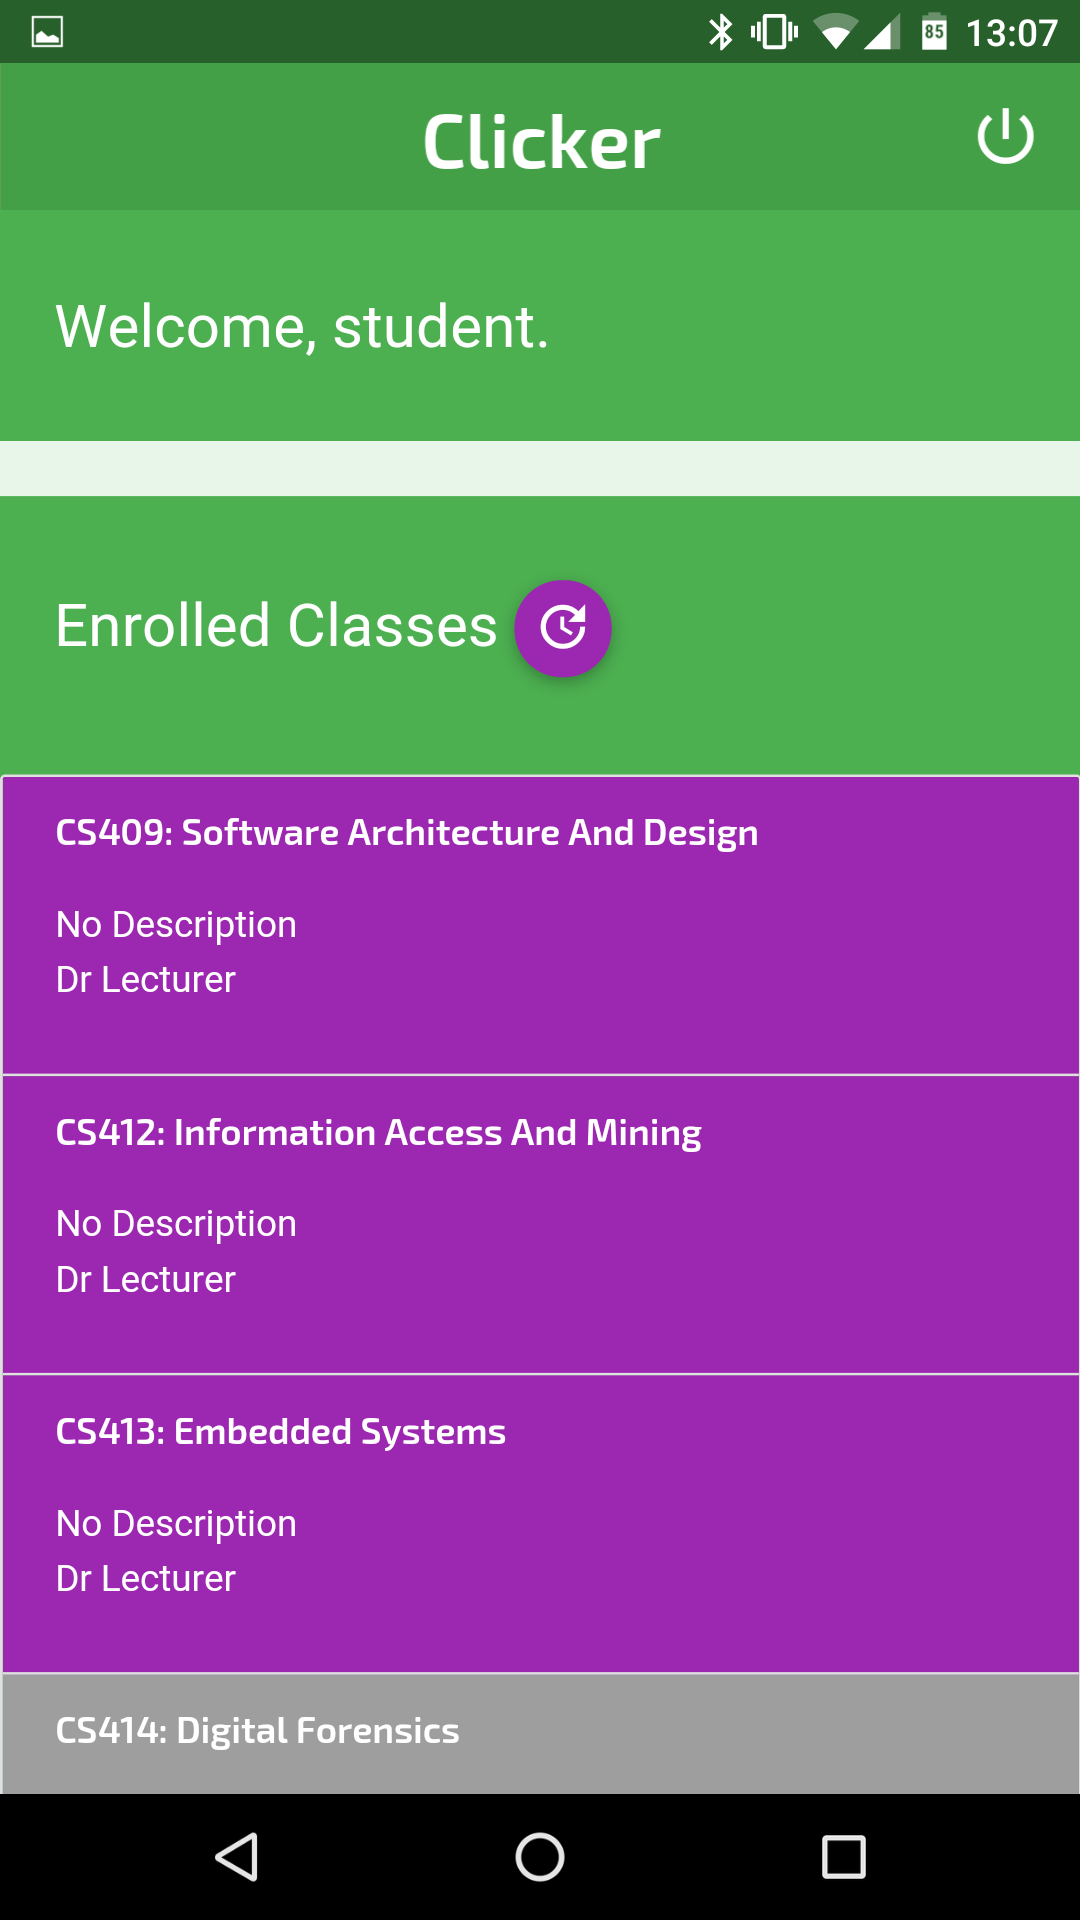
\includegraphics[width=3.1cm]{images/studenthome.png}
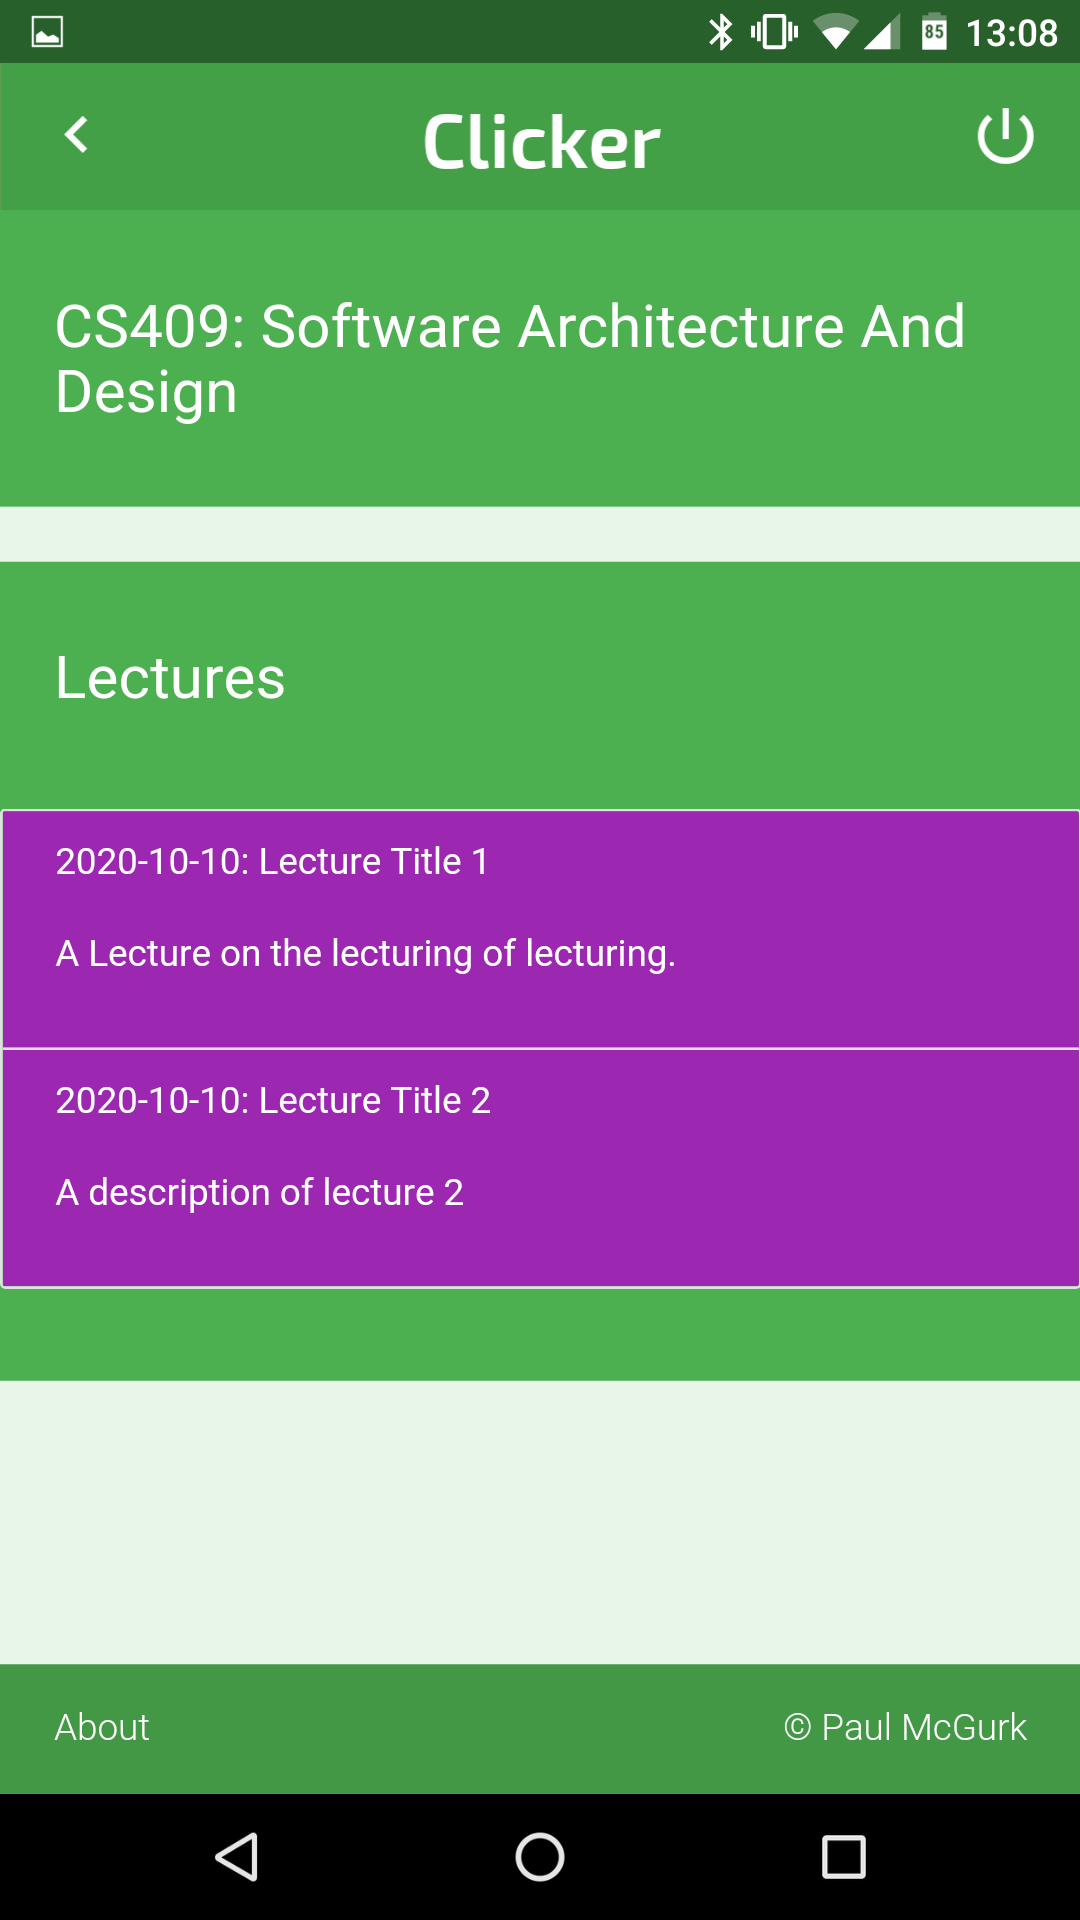
\includegraphics[width=3.1cm]{images/studentlectures.png}
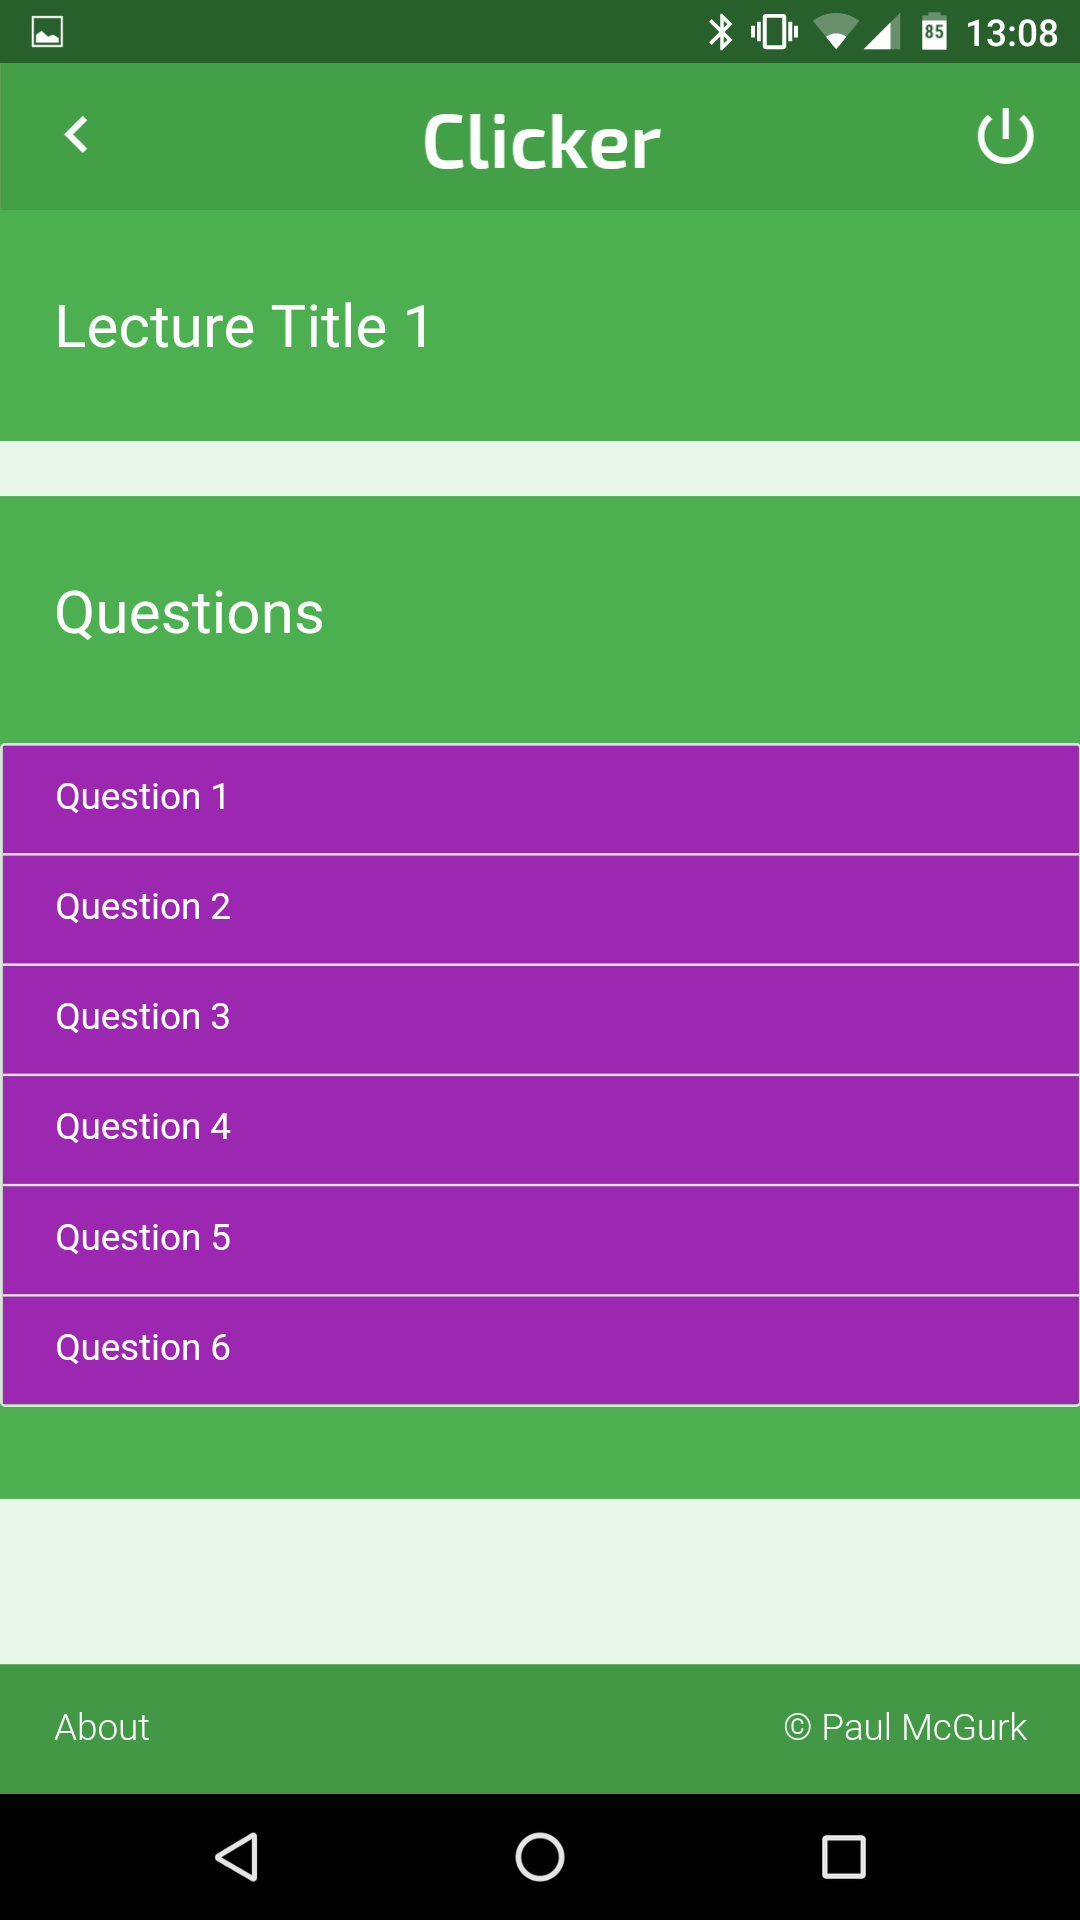
\includegraphics[width=3.1cm]{images/studentquestions.png}
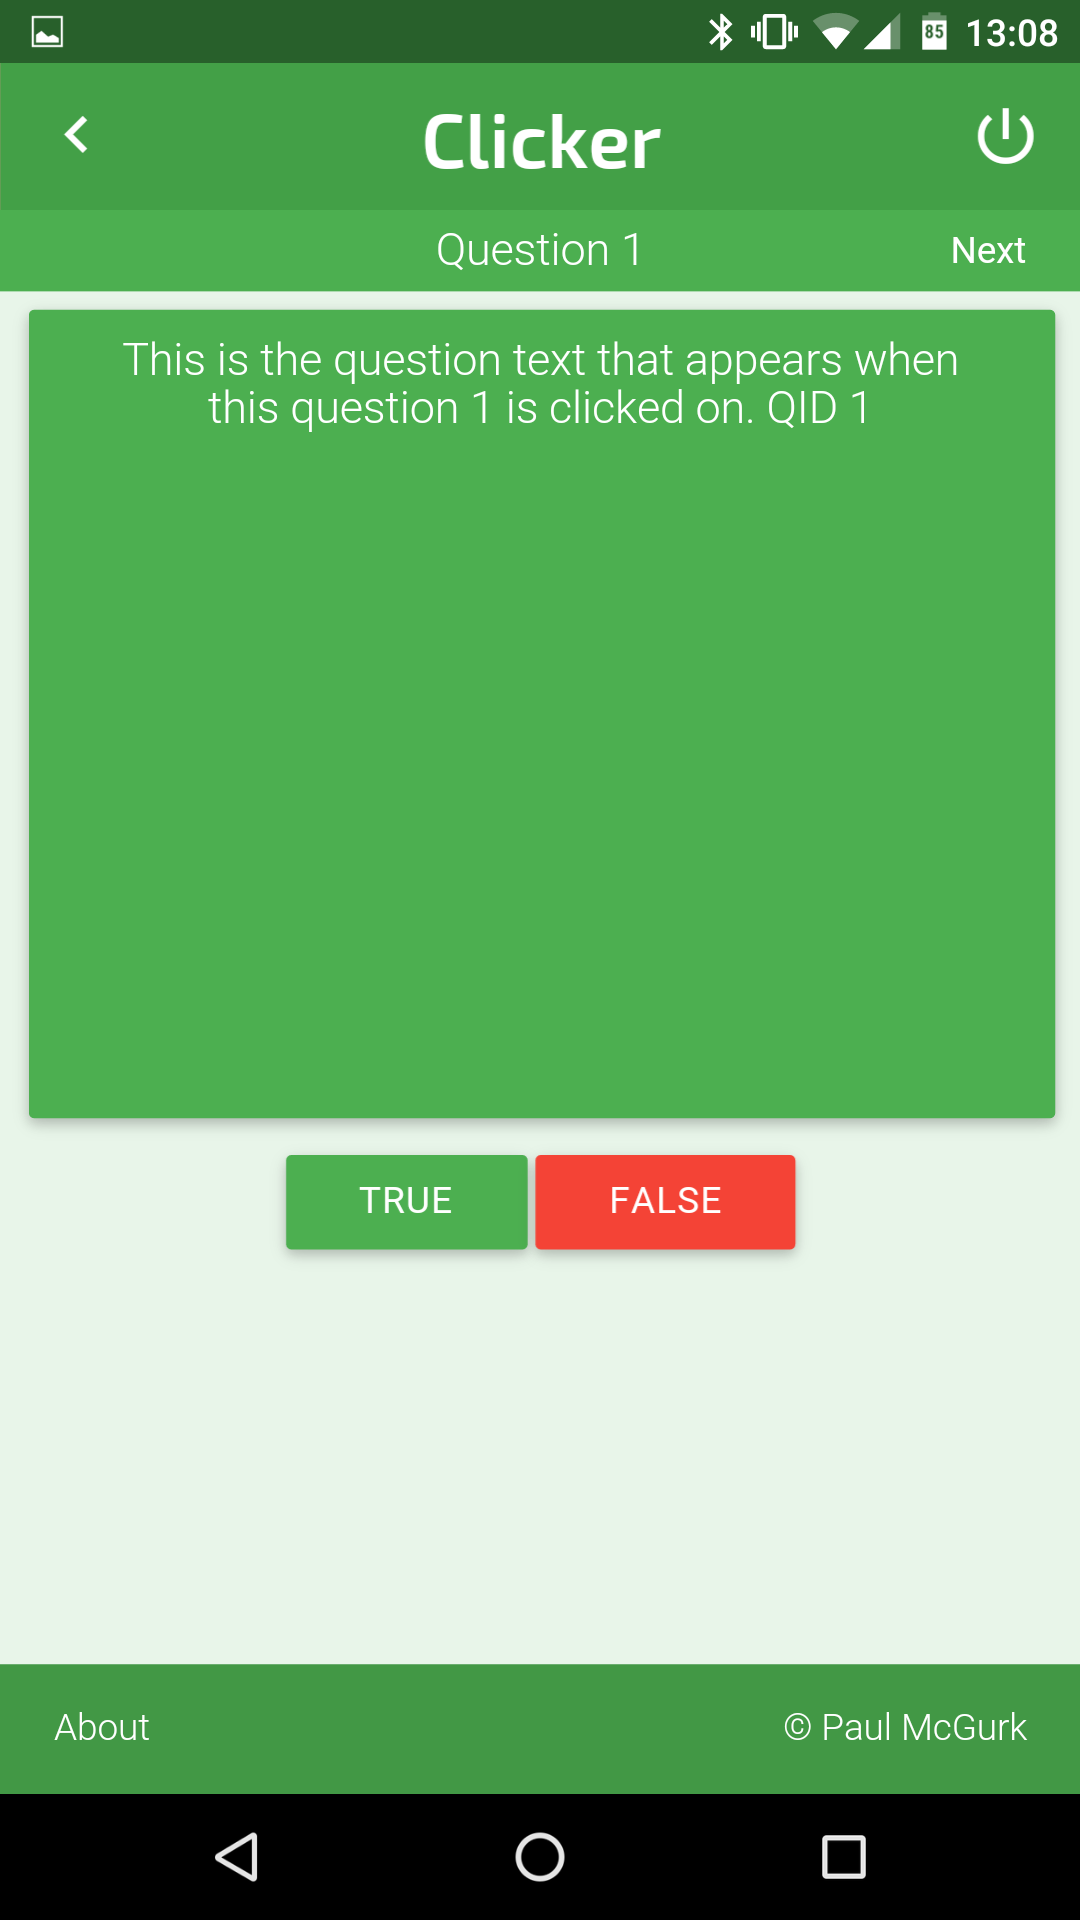
\includegraphics[width=3.1cm]{images/studentquestion.png}
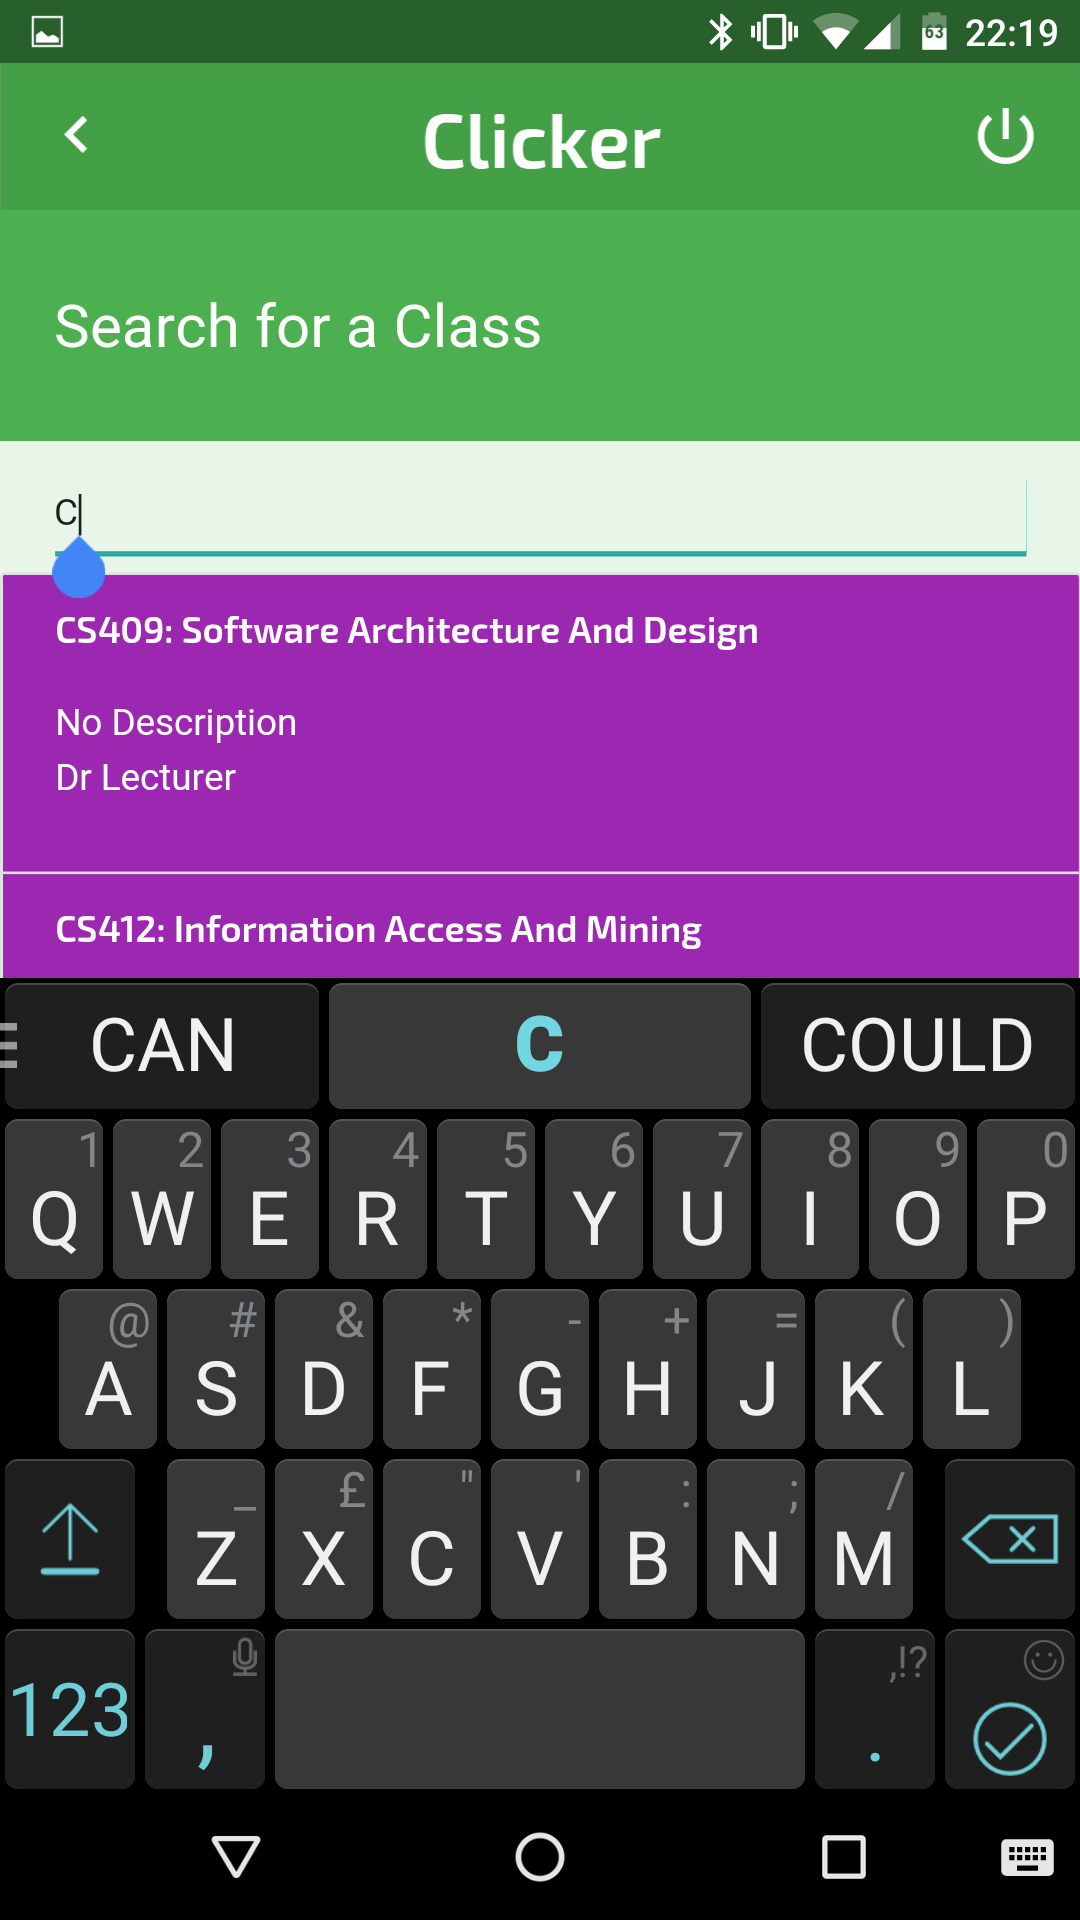
\includegraphics[width=3.1cm]{images/03021602.png}
\end{center}

These buttons submit the value of their selves to the database for comparison with the current answer value. It also adds an entity into the ``responses'' table, for use with the Lecturer's ``responses'' page, described below. There is also a page for searching for classes to join, but there is no mechanism for joining these classes at this moment.

\subsubsection{Lecture Side}
Similar to the student application, but shows classes which the lecturer owns with options to edit the classes/lectures/questions featured throughout. Currently, there is no way of editing  other than to do it manually in the database. There is also a ``responses'' page where lecturers can see responses to their questions using Chart.js.

\begin{center}
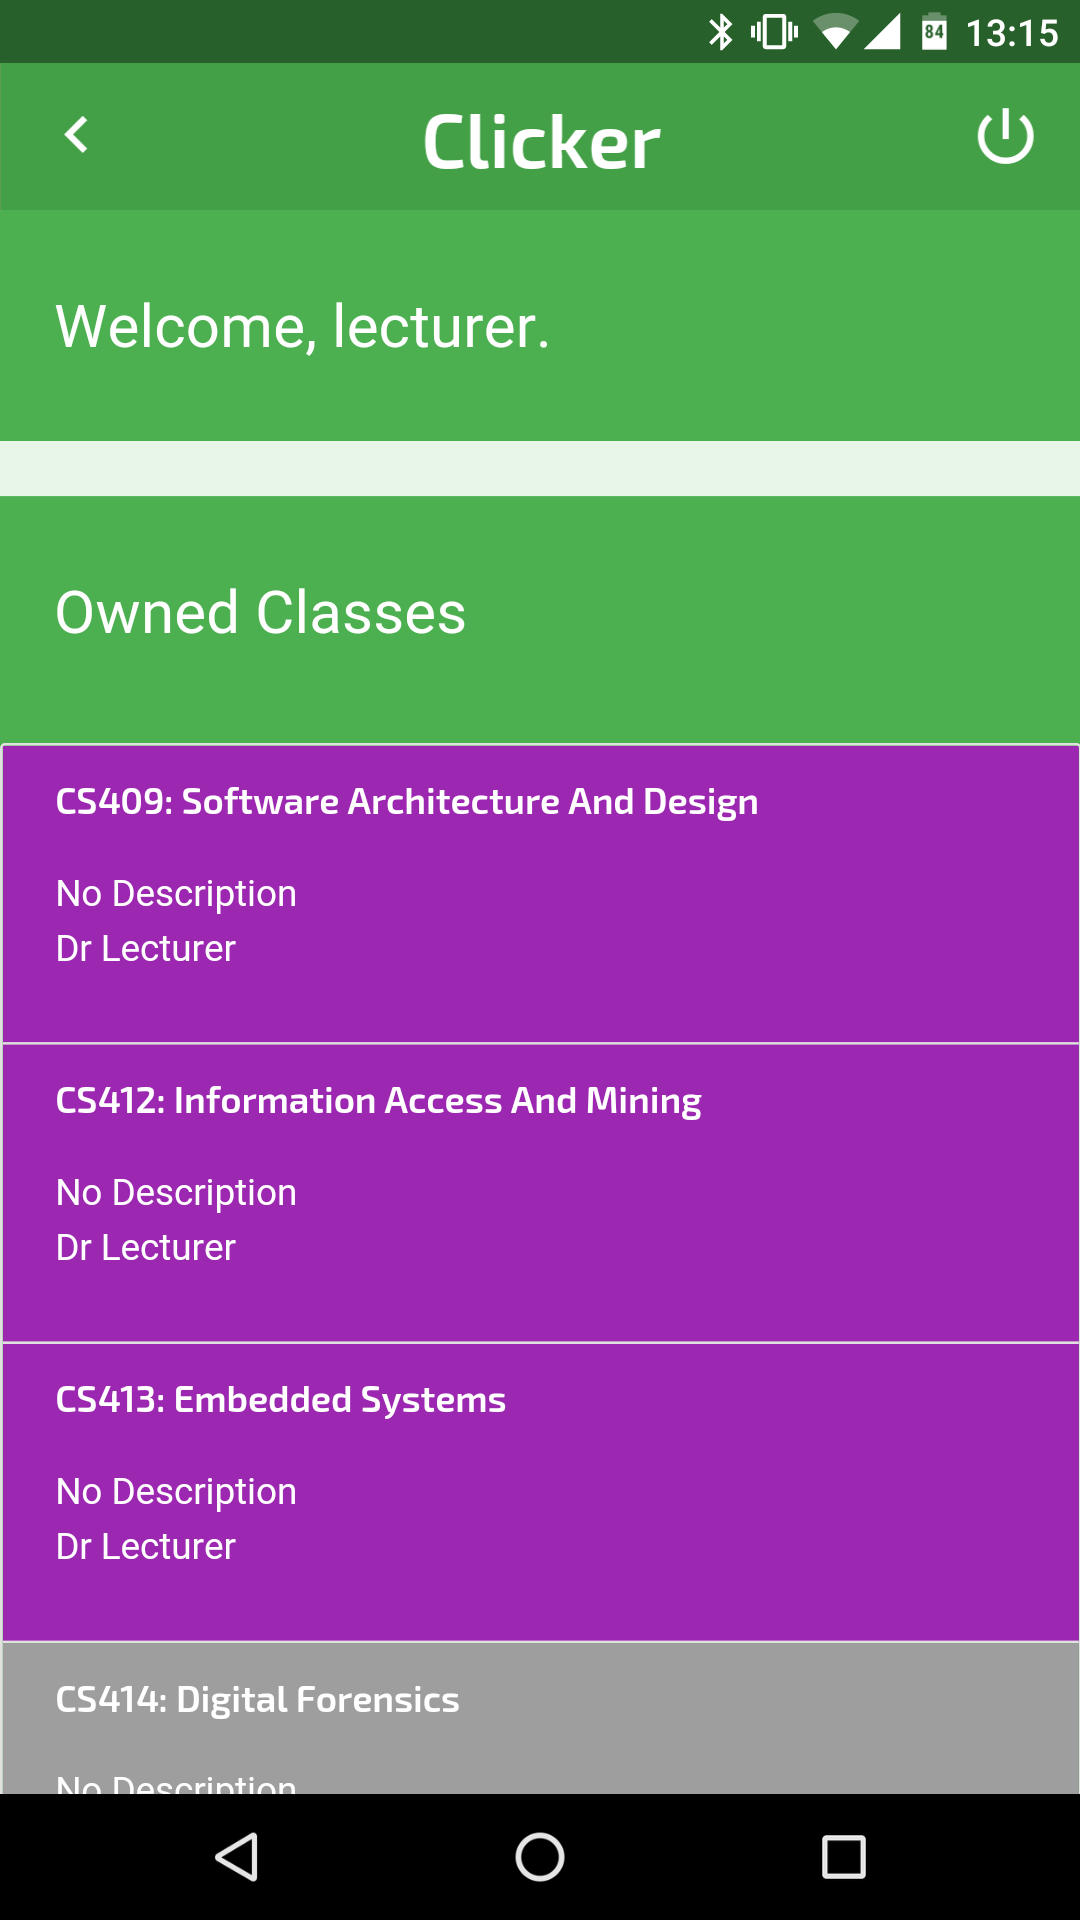
\includegraphics[width=3.1cm]{images/lecturerhome.png}
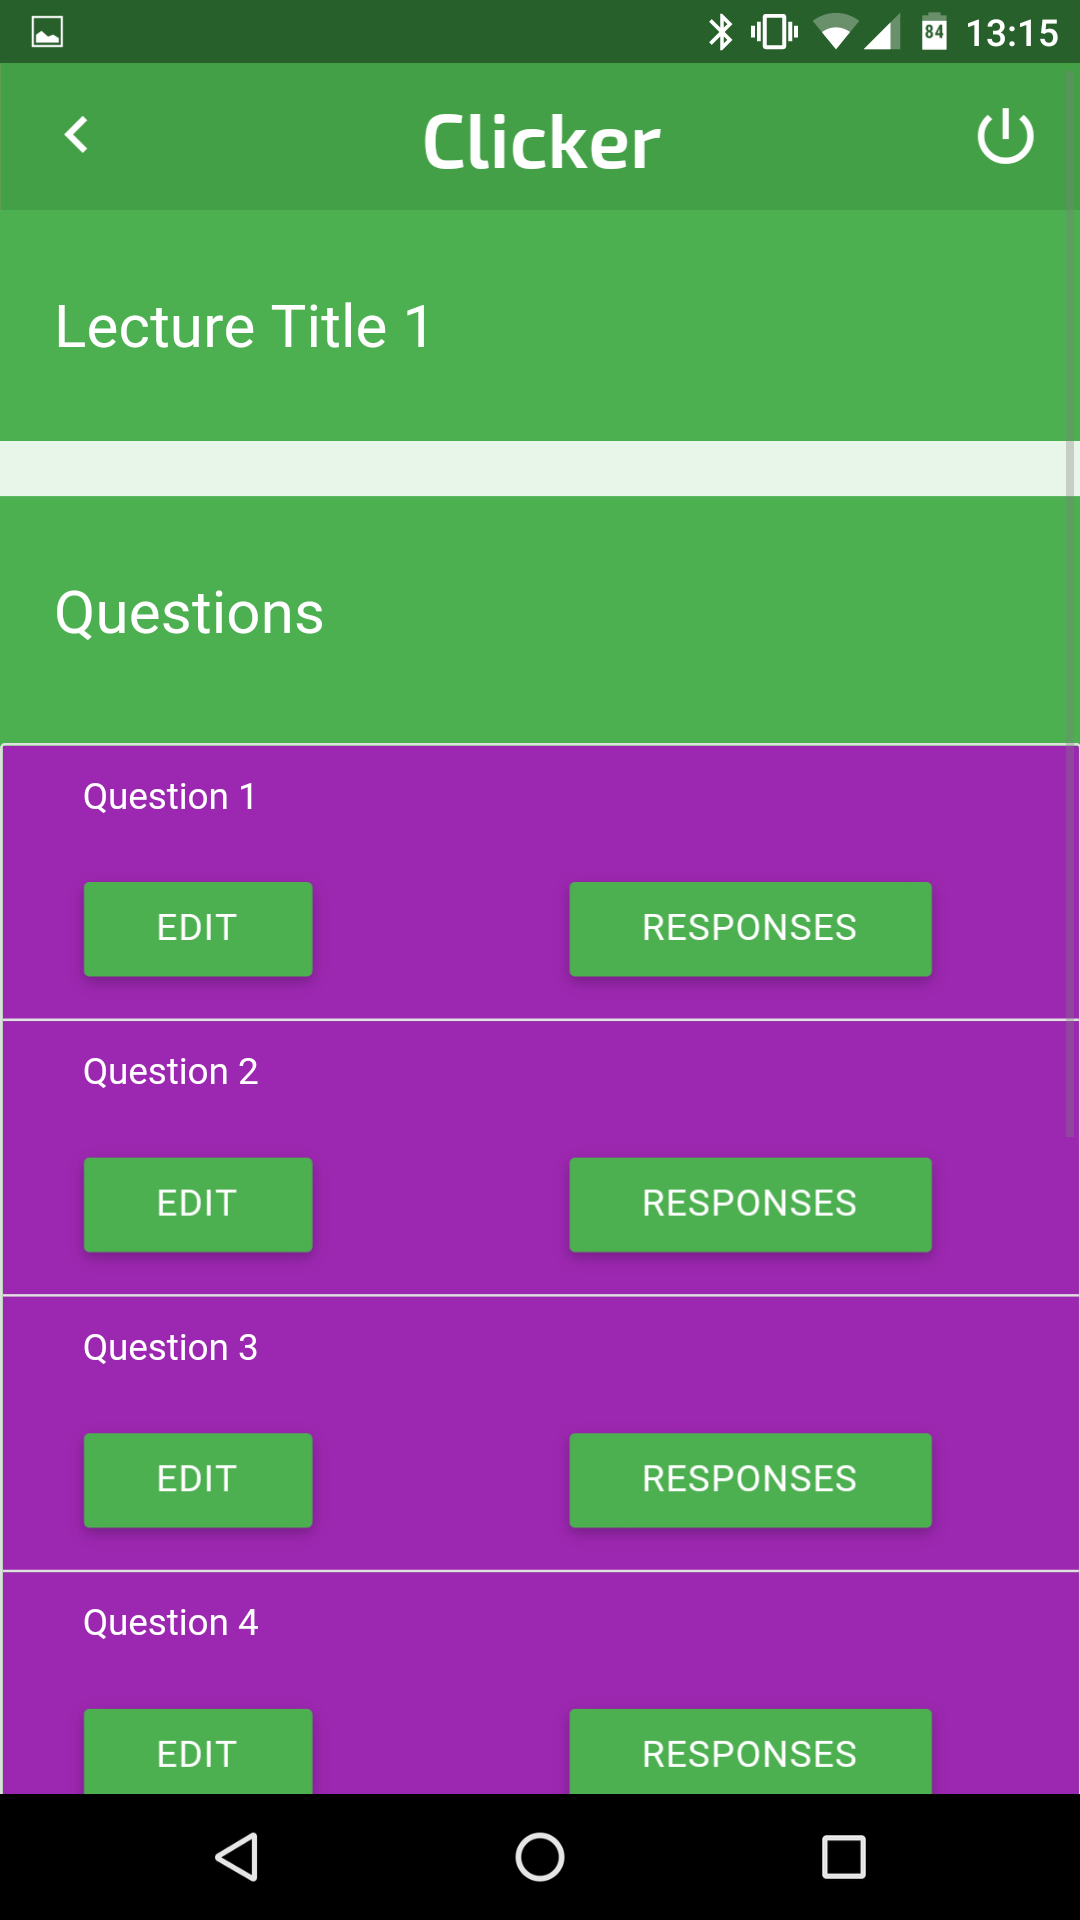
\includegraphics[width=3.1cm]{images/lecturerlectures.png}
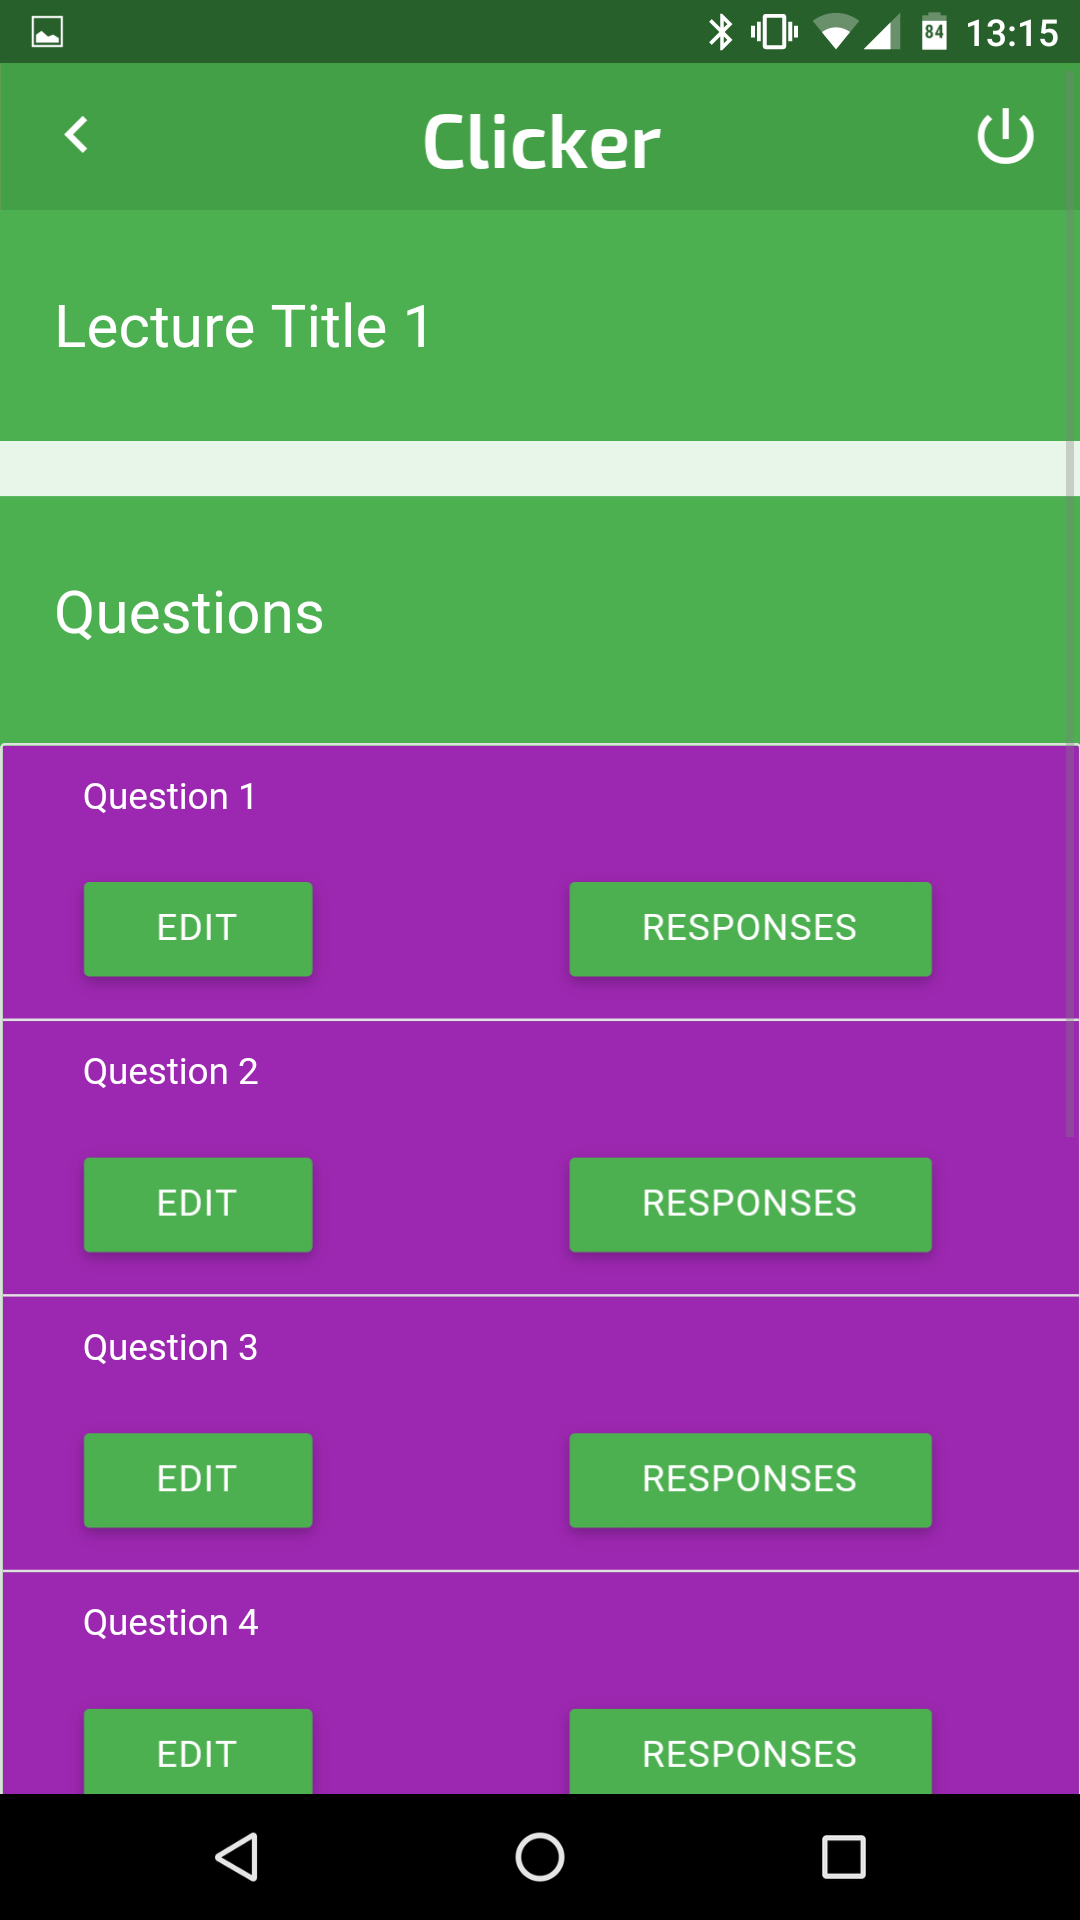
\includegraphics[width=3.1cm]{images/lecturerquestions.png}
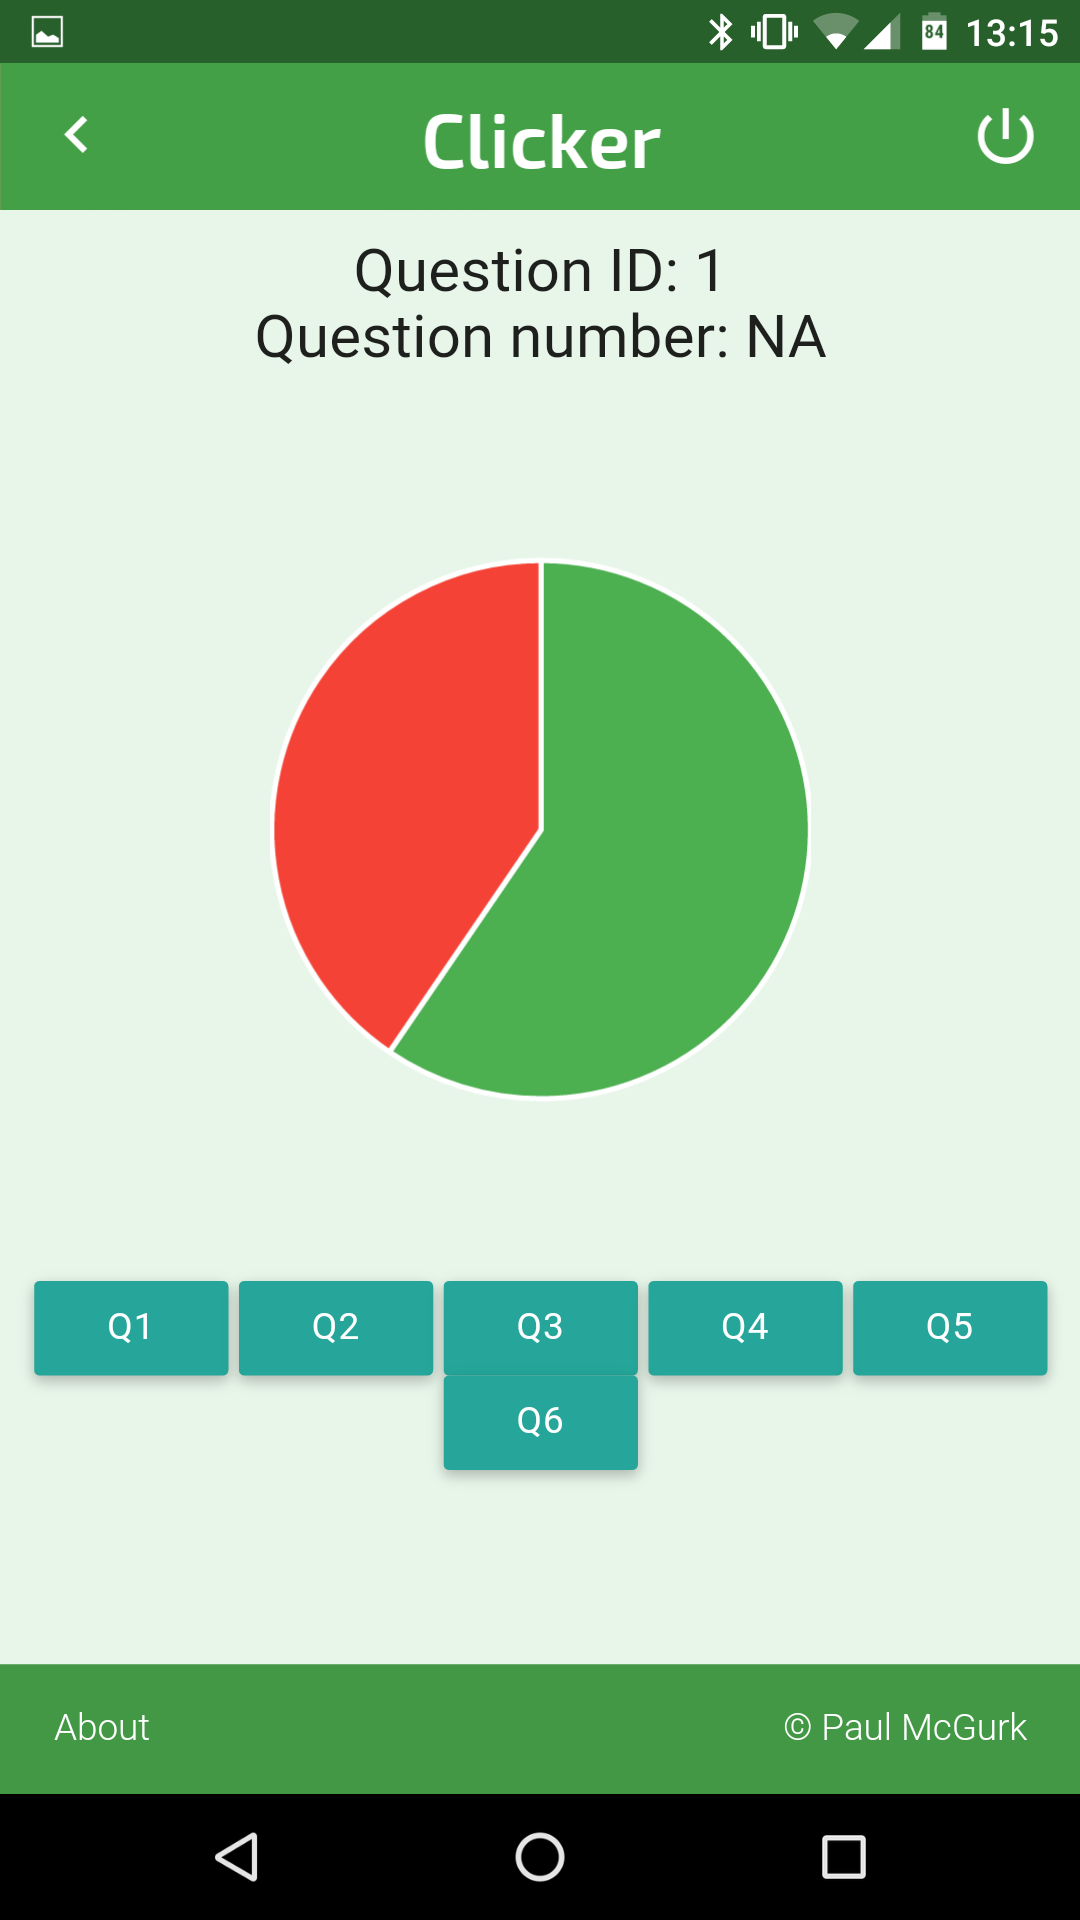
\includegraphics[width=3.1cm]{images/lecturerresponse.png}
\end{center}

\subsection{Alterations}
\subsubsection {Wi-Fi Direct}
After attempts to get wifi direct to do what is required of it for use as an access point to host this Web Application, it appeared that it had a lot of issues performing this. An alternative to this was also tested, ``HostAPD'', which turns the Raspberry Pi into a Wi-Fi access point, but there was also issues with this to do with constant disconnecting, and possible issues with user's devices not being able to access the internet when connected to this device, which is undesirable.

At this point, the likely implementation is a remote server hosting the Web Application, with students accessing it via their web browsers like a normal website. This implementation also allows for even less dedicated hardware to be used in the setup of this service, which is an aim of this project. However, I will continue to look for solutions to allow the use of a Raspberry Pi as an option.

\subsubsection{Dotti Display}
There was an issue with obtaining a dotti display for use in visualisation. However, after discussion with Marc Roper about alternatives, it was decided that an additional page in the Lecturer Application could be used to display the information in a more flexible way, using some sort of data visualisation library, namely, D3.js. 

There was an issue with D3.js being unsuitable due to using SVGs which aren't resolution dependent, and possibly being overkill for what is relatively simple data, so Chart.js was found as an alternative. This also allows even less dedicated hardware to be used in the service.

\subsection{Plan Going Forward}
The plan at the moment is to finish the application to a usable level. At this point, there is just a few things that need implemented, including:
\begin{itemize}
  \item Lecturer ability to create and edit classes.
  \item Responses page to update in real time rather than just on load.
  \item Student ability to join classes.
  \item More research into using a Raspberry Pi as the host, possibly in addition to remote host version of application.
\end{itemize}

This should be done within the first half of February, no later than the 10th, leaving plenty of time for evaluation and changes that come from it.

After a usable version of the application is finished, evaluation will be of the main importance. Getting a concrete plan for the evaluation and applying for ethics, and after the evaluation, modifying the application on the feedback to make it as useful and as user friendly as possible. 

There will also need to be extensive compatibility testing on as wide range of devices as I can, most notability, different Android versions, different browsers on each device, devices with varying screen sizes from extreme large to extreme small, and a wide range of Apple devices, but changes to the application should be minimal from these tests, as the framework used is very portable.

\newpage
\section{Report Structure}
\section{Title Page}
A title page with all required information

\section{Abstract}
A abstract describing the issues with modern clickers, etc.

\section{Acknowledgments}
A list of acknowledgments for the project.

\section{Table of Contents}
Table of contents.

\section{Introduction}
An introduction to the project
\subsection{Aim}
The aim for the project.

\section{Related Work}
\subsection{Justification for Chosen Applications}
A list of chosen comparative applications to compare to, if I go this way.

\subsection{Related Work 1}
\subsubsection{Strengths}
The strengths of a related work.

\subsubsection{Weaknesses}
The weakness of a related work.

\section{Problem description and specification}
A description of the problem and the specification

\section{System design}
A description of how I developed the project, and the technology used.

\section{Detailed design and implementation}
A detailed description of how the project works for maintenance, etc.

\section{Verification and validation}
Verification and validation of the project

\section{Results and evaluation}
Results and evaluation of the project

\section{Summary and Conclusions}
Summing up of the project and what I conclude from it.

\section{Appendices}
\subsection{User Guide}
\subsubsection{Admin}
A guide on setting up the application for the system administrator, including dependencies, database structure etc.

\subsubsection{Lecturer}
A guide on using the application for lecturers, including create a class, editing a class, adding lectures, adding questions, etc.

\subsubsection{Student}
A guide on using the application for students, including joining a class, answering questions, etc.

\subsection{Log Book}
Embedded log book


\newpage
\section{Meetings}
\subsubsection{30/10/15}
Initial meeting, discussed visions for implementation.

\subsubsection{06/11/15}
Discussion about project spec and plan.

\subsubsection{13/11/15}
Discussion about issues with wi-fi direct, limits, compatibility and usefulness, etc.

\subsubsection{26/11/15} 
Issues with dotti availability, possible homebrew alternatives. Discussed how connection method is not critical at this point, and focus should be on developing the application.

\subsubsection{02/11/15}
Discussed evaluation, which is to be done with a live preview in a real setting.
Possible initial data gathering through use of surveys to lecturers to see issues with ``clickers''.

\subsubsection{03/12/15}
Talked project spec/plan. Evaluation ideas mainly.

\subsubsection{05/01/16}
Discussed evaluation and progress. HostAPD may be out of the question, but alternative uses of pi was discussed.
Evaluation was discussed, likely after a prototype is developed. Aim for end of January.

\subsubsection{29/01/16}
More discussion on evaluation, going with the idea of a live lecture environment. Also discussed progress report.

\end{document}